\chapter{Работа с очередями FIFO}

\emph{Интерфес FIFO. Асинхронных режим. Режимы работы FIFO: Standard и First Word Fall Through. Интерфейс AXI Stream.}

\section{Содержание главы}

Основной литературой по FIFO является PG057. Требуется:
\begin{itemize}
\item описать всю последовательность действий по созданию и кастомизации ядра FIFO, а также включению его в код на VHDL, сделав при этом упор на интерфейс \emph{Native} и на интерфейс \emph{AXI4-Stream} (про интерфейс AXI4 Memory Mapped достаточно упомянуть);
\item написать testbench для ядра FIFO, чтобы показать его функциональность (т.е. то, как ядро работает), привести пример временных форм сигналов из симулятора;
\item описать принцип работы FIFO (описать два указателя~-- на начало и конец очереди в памяти, когда и как они увеличиваются и т.д.);
\item написать, отладить и описать VHDL-код усредняющего FIFO. Обязателен testbench.
\end{itemize}

\section{Что такое FIFO? VHDL-код FIFO на основе \\  регистров.}

\begin{figure}[h]
\centering
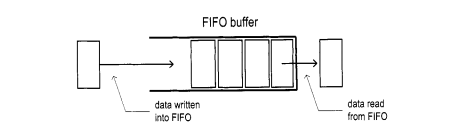
\includegraphics[width=0.6\textwidth]{fifo_bufer}
\caption{Концептуальная схема буфера FIFO}
\label{fifo_bufer_label}
\end{figure}

Буфер FIFO (first-in-first-out) является «эластичным» хранилищем между двумя подсистемами, как показано на концептуальной диаграмме рисунка 1.1.  Он имеет два управляющих сигнала, wr и rd, для операций записи и чтения. Когда wr устанавливается в '1', входные данные записываются в буфер. Операция чтения несколько вводит в заблуждение. Голова буфера FIFO всегда доступна и, следовательно, может быть прочитана в любое время. На самом деле сигнал rd действует как сигнал «удалить». Когда это утверждается, первый элемент (то есть голова) буфера FIFO удаляется, и становится доступным следующий элемент. Буфер FIFO является критическим компонентом во многих приложениях, и оптимизированная реализация может быть довольно сложной. В этом подразделе мы вводим простые,  кольцевые рисунки на основе циклических очередей.

\subsection{Реализация на основе циклических очередей}
Одним из способов реализации буфера FIFO является добавление схемы управления к регистровому файлу. Регистры в регистровом файле располагаются в виде круговой очереди с двумя указателями. Указатель записи указывает на начало очереди, а указатель чтения указывает на хвост очереди. Указатель продвигает одну позицию для каждой операции записи или чтения. Операция кольцевой очереди из восьми слов показана на рисунке 1.2.
	Буфер FIFO обычно содержит два сигнала состояния, полный и пустой, чтобы указать, что FIFO заполнен (т.е. не может быть записан) и пуст (т.е. не может быть прочитан) соответственно. Одно из двух условий возникает, когда указатель чтения равен указателю записи, как показано на рис. 1.2 (a), (f) и (i). Самая сложная задача разработки контроллера - получить механизм, позволяющий отличать два условия. Одна из схем заключается в использовании двух триггеров  для отслеживания пустых и полных статусов. Триггеры устанавливаются в '1' и '0' во время инициализации системы, а затем изменяются в каждом такте в соответствии со значениями wr и rd сигналов. Код показан в ниже:

\begin{figure}[h]
\centering
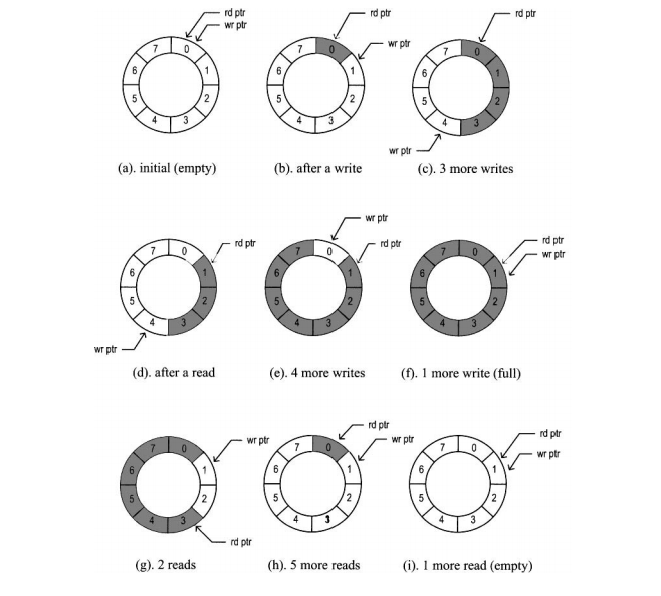
\includegraphics[width=1.1\textwidth]{circular_queue}
\caption{Буфер FIFO, основанный на кольцевой очереди.}
\label{circular_queue_label}
\end{figure}

\lstinputlisting[caption=FIFO bufer, label=fifo_kur]{fifo_kur.vhd}

Код разделен на регистровый файл и контроллер FIFO. Контроллер состоит из двух указателей и двух статусных триггеров. Его логика следующего состояния исследует сигналы wr и rd и предпринимает соответствующие действия. Например, рассмотрим случай «10», из которого следует, что происходит только операция записи. Сначала проверяется статус триггера, чтобы убедиться, что буфер не заполнен. Если это условие выполняется, мы продвигаем указатель записи на одну позицию и очищаем пустой статус триггер. Хранение одного дополнительного слова в буфере может сделать его полным. Это происходит, если новый указатель записи «ловит» указатель чтения, который задается выражением w\_ pt\_r succ = r\_ ptr\_reg.

\subsection{Схема проверки}

Схема проверки проверяет работу  $2^{3} \times 3$ FIFO буфера. Мы используем три переключателя для генерации входных данных и используем две кнопки для wr и rd сигналов. 3-разрядное считывание состояния полного и пустого сигнала состояния отображаются в пяти дискретных светодиодах. Исходными входами кнопок являются btn (0) и btn (I), а ослабленные сигналы - db\_btn (0) и db\_btn (l). Код показан в листинге 1.2.

\lstinputlisting[caption=Testing circuit for a FIFO buffer, label=fifo_testing]{fifo_testing.vhd}

\section{FIFO IP}

 \noindent 
\textbf{Шаг 1: открываем проект} \\ 
\\
Считаю что данный шаг не стоит описывать подробно, так как вы неоднократно выполняли данную процедуру.\\
\\
\textbf{Шаг 2: Настройка генератора FIFO}
\begin{enumerate} 
\item Выберите IP Catalog во вкладке  Flow Navigator. 
\itemНажмите IP Catalog и он отобразится в новой вкладке.
\itemНажмите папку Memories \& Storage Element, затем FIFOs. Выберите FIFO Generator. Альтернативный способ написать в строке поиска fifo.
\begin{figure}[h]
\centering
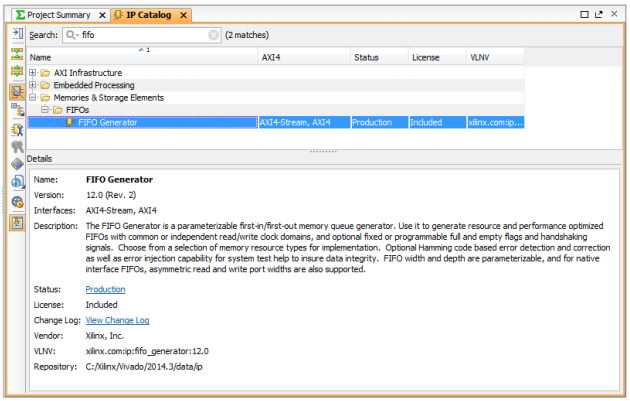
\includegraphics[width=1.1\textwidth]{fifo_ip_1}
\caption{ Customize IP}
\label{fifo_ip_1_label}
\end{figure}
\itemЩелкните правой кнопкой мыши и выбирете Customize IP, или дважды щелкните на FIFO Generator. Откроется окно настройки генератора FIFO.
\begin{figure}[h]
\centering
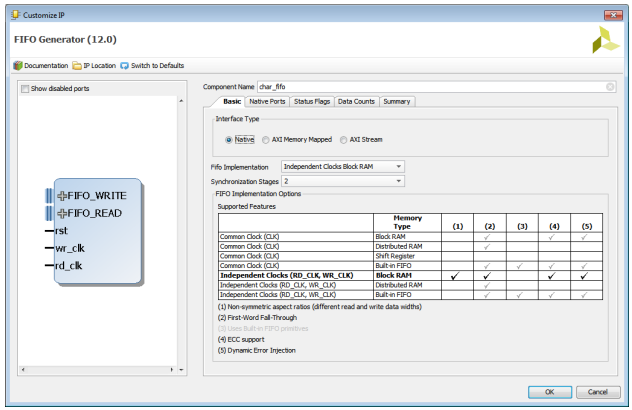
\includegraphics[width=1.1\textwidth]{fifo_ip_2}
\caption{Xilinx IP Catalog – FIFO Core}
\label{fifo_ip_2_label}
\end{figure}
\item Выберите тип интерфейса Native.
\item Установить режим чтения Standart FIFO.
\itemЗадайте Write Width, Write Depth, Read Width.
\itemПерейдите во вкладку Status Flags, в разделе Read Port Handshaking установите галочку в Valid Flag.
\itemУбедитесь, что информация верна, как показано, и нажмите «ОК».
\end{enumerate}

\textbf{Шаг 3: Создание выходных продуктов} \\ 

После завершения настройки IP-адреса откроется диалоговое окно «Generate Output Products», как показано на следующем рисунке. Выходными продуктами для IP являются различные файлы, необходимые для поддержки использования IP в synthesis, simulation, and implementation. 
\begin{enumerate} 
\begin{figure}[h]
\centering
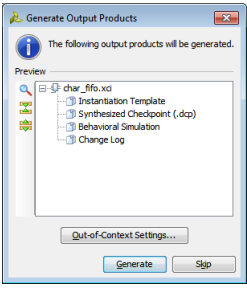
\includegraphics[width=0.4\textwidth]{fifo_ip_3}
\caption{Generate Output Products}
\label{fifo_ip_3_label}
\end{figure}
\itemНажмите «Generate», чтобы создать требуемые выходные продукты (рис 1.5).\\
По умолчанию среда IDE Vivado создает файл Synthesized Checkpoint (DCP). Создание DCP показано на следующем рисунке:
\begin{figure}[h]
\centering
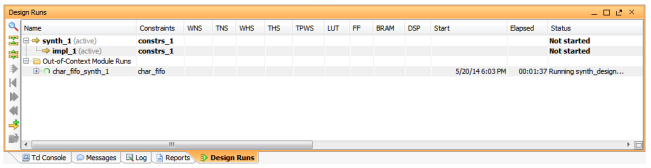
\includegraphics[width=1.1\textwidth]{fifo_ip_4}
\caption{Out-of-Context Synthesis Run}
\label{fifo_ip_4_label}
\end{figure}
\item На вкладке «Ip Source»  в окне «Source» просмотрите выходные продукты, созданные для настройки генератора FIFO. Если вы не создали выходные продукты, они будут автоматически генерироваться при запуске синтеза верхнего уровня. (рис 1.6)
\item Изучите консоль Tcl в среде IDE Vivado, как показано на следующем рисунке, и просмотрите команды Tcl, используемые для добавления ядра генератора FIFO в ваш проект. (рис 1.7)
\begin{figure}[h]
\centering
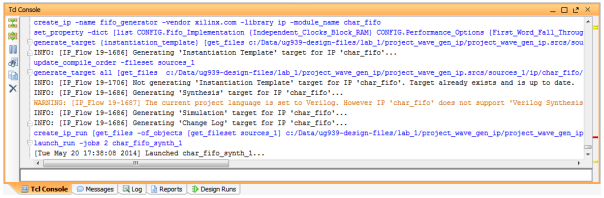
\includegraphics[width=1.1\textwidth]{fifo_ip_7}
\caption{Tcl Console Commands for Adding IP}
\label{fifo_ip_7_label}
\end{figure}
\end{enumerate} 

\begin{itemize}
\itemКоманда create\_ip добавляет IP в текущий проект.
\itemКоманда set\_property задает различные параметры конфигурации, выбранные в диалоговом окне «Настройка IP».
\itemКоманда generate\_target создает заданные выходные продукты для настроенного IP.
\itemКоманда create\_ip\_run создает синтез вне контекста для настроенного IP.
\end{itemize}

\textbf{Шаг 4: Создание IP-адреса в проекте} \\ 
Теперь вы создадите экземпляр настройки IP в проекте, скопировав и вставив шаблон верификации VHDL в соответствующий исходный файл VHDL в своем проекте и изменив сигналы.
\begin{enumerate}
\itemНа вкладке «Ip Source»  в окне «Source» разверните шаблон создания шаблона и дважды щелкните файл, чтобы открыть шаблон в текстовом редакторе Vivado.
\itemПрокрутите вниз до строки 57 файла шаблона и выберите и скопируйте текст экземпляра модуля, как показано на следующем рисунке 1.8.
\begin{figure}[h]
\centering
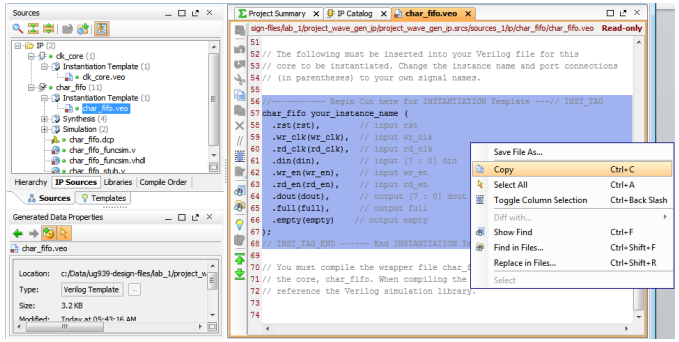
\includegraphics[width=1.1\textwidth]{fifo_ip_8}
\caption{FIFO Core Generator - Instantiation Template}
\label{fifo_ip_8_label}
\end{figure}
\itemЗатем вы вставляете шаблон инстанцирования в соответствующий исходный RTL-файл. В этом случае вы вставляете модуль в верхний уровень дизайна, в исходный файл vhd.
\itemНа вкладке «Hierarchy» в представлении «Sources» дважды щелкните файл .vhd, как показано на следующем рисунке, чтобы открыть этот файл для редактирования рис (1.9).

\begin{figure}[h]
\centering
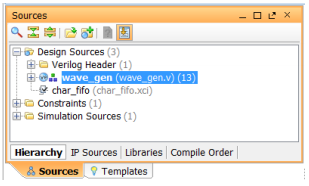
\includegraphics[width=0.4\textwidth]{fifo_ip_9}
\caption{Файл vhd}
\label{fifo_ip_9_label}
\end{figure}

\item Измените имена портов следующим образом, чтобы подключить порты модуля к дизайну (рис 1.10):

\begin{figure}[h]
\centering
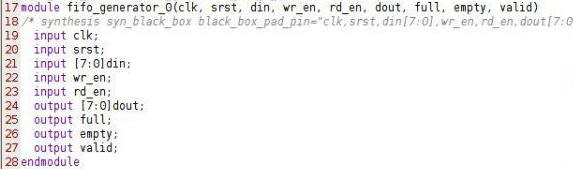
\includegraphics[width=0.4\textwidth]{fifo_ip_10}
\caption{Порты}
\label{fifo_ip_10_label}
\end{figure}

\item В меню боковой панели текстового редактора нажмите кнопку Save File, чтобы сохранить изменения в файле .vhd.
\end{enumerate}

\section{Интерфейс FIFO}

Ядро FIFO (first-in first-out - первый вошел, первый вышел) генератора может использоваться в любом приложении, требующем упорядоченного
хранения и извлечения, что позволяет создавать высокопроизводительные и оптимизированные по площади проекты.
Ядро обеспечивает оптимизированное решение для всех конфигураций FIFO и  максимальную производительность (до 500 МГц) при использовании
минимальных ресурсов.

Это ядро поддерживает Native интерфейс, AXI Memory Mapped и AXI4-Stream interface.
Оно может быть настроено с использованием модификаторов IP Vivado в каталоге
IP как завершенное решение с уже реализованной логикой управления, включая управление указателями
чтения и записи и генерацию флагов состояния.


\section{Оформление}

Очень хорошее и краткое введение в LaTeX можно найти в книге Столярова (\href{url}{http://www.stolyarov.info/books/latex3days/}).

\section{Заголовок 1-го уровня} 
\subsection{Заголовок 2-го уровня}
\subsubsection{Заголовок 3-го уровня}

Текст. Текст. Текст. \emph{Текст курсивом.} Поставить тире~-- вот так. Текст в "<кавычках">.

Чтобы сделать новый абзац, нужно пропустить строку.

Пример кода:

\begin{Code}
\begin{lstlisting}
library IEEE;
use IEEE.STD_LOGIC_1164.ALL;

entity Latch is
    port ( C : in  STD_LOGIC;
           D : in  STD_LOGIC;
           Q : out STD_LOGIC);
end Latch;

architecture Behavioral of Latch is
    signal q_tmp : std_logic := '0';
begin
    latch_process: process (C, D)
    begin
        if (C = '1') then
            q_tmp <= D;
        end if;
    end process;
    Q <= q_tmp;
end Behavioral;
\end{lstlisting}
\end{Code}

Пример кода в строке: \lstinline?С = 1?. Или вот так: \lstinline?S(7 downto 1) <= S(6 downto 0);?. Здесь код помещен между знаками вопроса.

Пример нумерованного списка:

\begin{enumerate}
\item Пункт 1.
\item Пункт 2.
\item Пункт 3.
\end{enumerate}

Пример ненумерованного списка:

\begin{itemize}
\item Пункт 1.
\item Пункт 2.
\item Пункт 3.
\end{itemize}

Вот так оформляется таблица с тремя колонками:

\begin{table}[h]
\centering
\begin{tabular}{|c|c|c|}
\hline
input               & \multicolumn{2}{c|}{output} \\ \hline
r                   & code        & active         \\ \hline
\texttt{1{-}{-}{-}} & \texttt{11} & \texttt{1}     \\
\texttt{01{-}{-}}   & \texttt{10} & \texttt{1}     \\
\texttt{001-}       & \texttt{01} & \texttt{1}     \\
\texttt{0001}       & \texttt{00} & \texttt{1}     \\
\texttt{0000}       & \texttt{00} & \texttt{0}     \\
\hline
\end{tabular}
\end{table}

Рисование осуществляется с помощью пакета 'TikZ':

\begin{figure}[ht]
\centering
\begin{tikzpicture}[>=latex']
\tikzstyle{arith_op} = [draw, fill=blue!20, circle, minimum size=2em]

% inputs
\node at (0,4) (input_a) {\texttt{a}};
\node at (0,3) (input_b) {\texttt{b}};
\node at (0,1) (input_c) {\texttt{c}};
\node at (0,0) (input_1) {\texttt{1}};

% operations
\node[arith_op] at (1,3) (block_plus_1) {$+$};
\node[arith_op] at (1,1) (block_plus_2) {$+$};
\node[arith_op] at (2,2) (block_minus) {$-$};

% connections
\draw[->] (input_a) -- (1,4) -- node {} (block_plus_1);
\draw[->] (input_b) -- node {} (block_plus_1);
\draw[->] (input_c) -- node {} (block_plus_2);
\draw[->] (input_1) -- (1,0) -- node {} (block_plus_2);
\draw[->] (block_plus_1) -- (2,3) -- node {} (block_minus);
\draw[->] (block_plus_2) -- (2,1) -- node {} (block_minus);
\draw[->] (block_minus) -- (3,2);
\end{tikzpicture}
\caption{Оптимизированная комбинационная схема.}
\label{label_fig_1}
\end{figure}

Ссылка на рисунок делается по \emph{label} вот так: \ref{label_fig_1}.

Вставка скриншотов программ (PNG) возможна следующим образом (файл изображения находится в папке с кодом):

\begin{figure}[h]
\centering
\includegraphics[width=0.6\textwidth]{test_fig}
\caption{Некий рисунок}
\label{test_fig_label}
\end{figure}
